%
% Magyar nyelvű szakdolgozatminta az Eszterházy Károly Katolikus Egyetem hallgatóinak.
% A matematika illetve informatika szakosok ne ezt, hanem a
% thesis-ekf-template-mat-inf.tex sablont használják!
%

\documentclass[
% opciók nélkül: egyoldalas nyomtatás, elektronikus verzió
% twoside,     % kétoldalas nyomtatás
% tocnopagenum,% oldalszámozás a tartalomjegyzék után kezdődik
]{thesis-ekf}
\usepackage[T1]{fontenc}
\PassOptionsToPackage{defaults=hu-min}{magyar.ldf}
\usepackage[magyar]{babel}
\footnotestyle{rule=fourth}
\usepackage{natbib,pdfpages}
\setcitestyle{aysep={}}

\begin{document}
\institute{Matematikai és Informatikai Intézet}
\title{Szervezet népszerűsítésének nyilvántartása webes eszközökkel}
\author{Kovács Norbert\\Programtervező Informatika}
\supervisor{Dr. Király Roland\\Egyetemi docens}
\city{Eger}
\date{2022}
\maketitle

\tableofcontents

\chapter*{Bevezetés}
\addcontentsline{toc}{chapter}{Bevezetés}
\section*{Miért}
\section*{Codeigniter}
\cite[27--28]{Bona}

\chapter{Adatbázis tervezése}
\cite[]{Gyorffy,Juhasz}

\chapter{Codeigniter 3}
\cite[]{Gyorffy,Juhasz}

\chapter{Ion auth 3}
\section{jogosultsági rendszer tervezése}
\cite[]{Gyorffy,Juhasz}

\chapter{Bootstrap}
\cite[]{Gyorffy,Juhasz}

\chapter{Felhasználói felület}
\cite[]{Gyorffy,Juhasz}

\chapter{Üzembe helyezés}
\cite[]{Gyorffy,Juhasz}

\chapter*{Összegzés}
\addcontentsline{toc}{chapter}{Összegzés}

\begin{thebibliography}{}
\addcontentsline{toc}{chapter}{\bibname}
\bibitem[Bóna(1998)]{Bona}
Bóna István 1998. \emph{Az Árpádok korai várai}. Ethnica Kiadó. Debrecen.
\bibitem[Györffy(1970)]{Gyorffy}
Györffy György 1970. \emph{A honfoglaló magyarok települési rendjéről}. Archeologiai Értesítő 97: 191--242.
\bibitem[Juhász(1988)]{Juhasz}
Juhász Dezső 1988. \emph{A magyar tájnévadás}. Nyelvtudományi Értekezések 126. Akadémiai Kiadó. Budapest.
\end{thebibliography}

% Aláírt, szkennelt nyilatkozat beillesztése a szakdolgozat végére
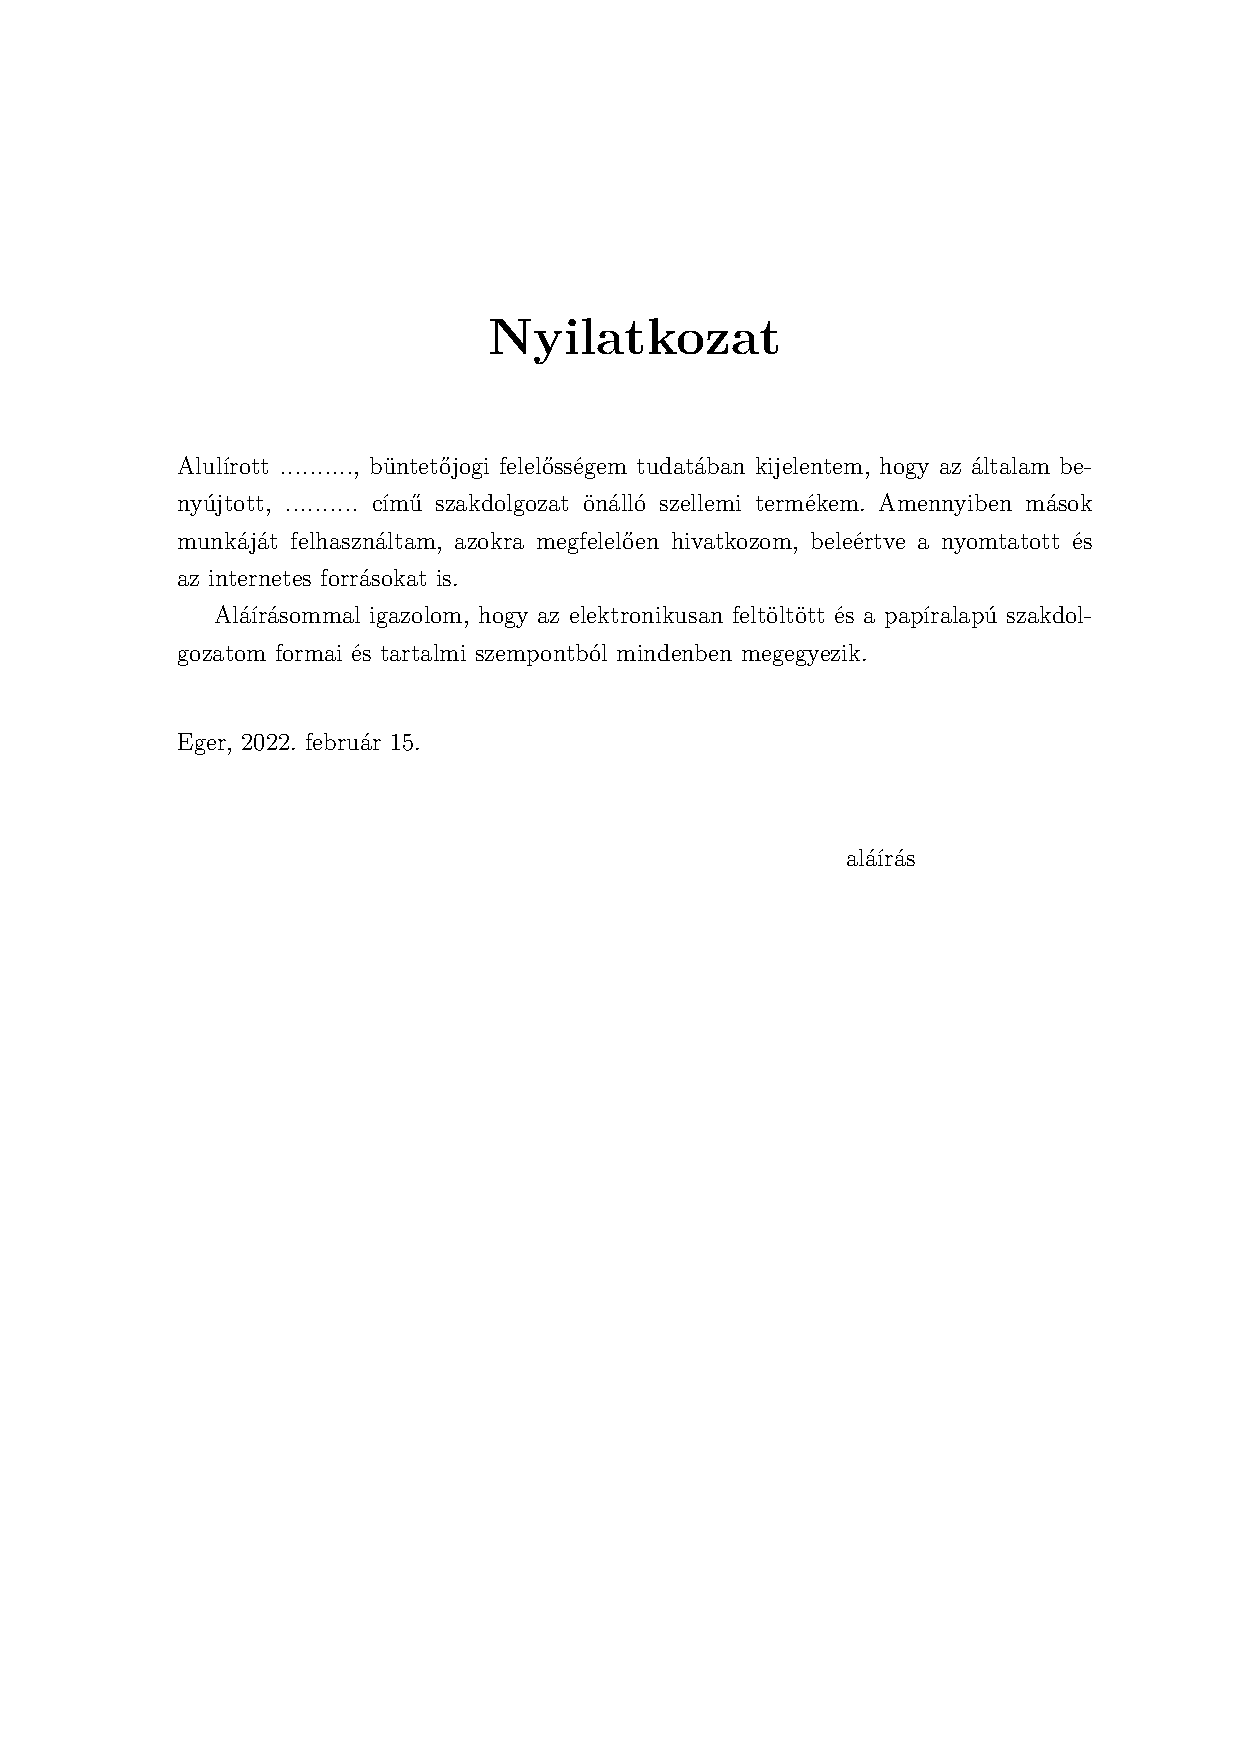
\includepdf[pagecommand={\thispagestyle{empty}}]{nyilatkozat.pdf}
\end{document}